\chapter{Thí nghiệm và thảo luận}
\thispagestyle{fancy}

\section{Thí nghiệm}

\subsection{Xữ lí dữ liệu}
\begin{itemize}
    \item Dữ liệu sử dụng thu thập từ 44 người theo bộ dữ liệu MIT-BIH với những độ tuổi và giới tính khác nhau, kèm theo đó là những ghi chú về nhịp tim của bệnh nhân bao gồm: Độ tuổi, giới tính, thuốc đang sử dụng, những điểm đặc biệt trong bản ghi của bệnh nhân,...
    \item Một số dữ liệu không được sử dụng trong quá trình nghiên cứu là: 102, 104, 107, 217 do những bệnh nhân này có sử dụng máy trợ tim (peatmaker) nên nhịp tim không tự nhiên ảnh hưởng đến quá trình phân loại theo nhiều nghiên cứu trước đây.
    \item Dữ liệu trong thử nghiệm chỉ lấy trên chuyển đạo II (ML II) trong 2 channel của dữ liệu MIT-BIH (channel 1) vì chuyển đạo này thể hiện rõ ràng nhất đặc điểm cơ bản của ECG.\cite{something}
    \item Dữ liệu được thu thập với tốc độ lấy mẫu là 360 mẫu/s. Một bản ghi từ một bệnh nhân được ghi lại trong 30 phút 5 giây. Một bản ghi có 650 000 mẫu.
    \item Sau khi trích xuất đặc trưng khoảng R-R và chuẩn hóa về cùng hình dạng thì mỗi khoảng R-R có độ dài là 324.
\end{itemize}

\subsection{Phân loại trên 1 đoạn RR}
\subsubsection{Chia tập dữ liệu}
\begin{center}
    \begin{tabular}{|c|c|}
    \hline 
    Tập dữ liệu huấn luyện & Tập dữ liệu kiểm thử \\ 
    \hline 
    81149 & 22399\\
    \hline 
    \end{tabular}
\end{center}

\subsubsection{Kết quả}
Kết quả được đánh giá theo độ đo: Precision, Recall, F1-score, Accuracy, Loss.
\begin{center}
    \begin{tabular}{|c|c|c|}
    \hline
    Estimate & Normal & Abnormal\\
    \hline 
    Precision & 0.96 & 0.74\\ 
    \hline 
    Recall & 0.87 & 0.92\\
    \hline 
    F1-score & 0.90 & 0.81\\
    \hline 
    Accuracy & \multicolumn{2}{|c|}{0.95} \\
    \hline 
    Loss & \multicolumn{2}{|c|}{0.03} \\
    \hline
    \end{tabular}
\end{center}
\begin{center}
    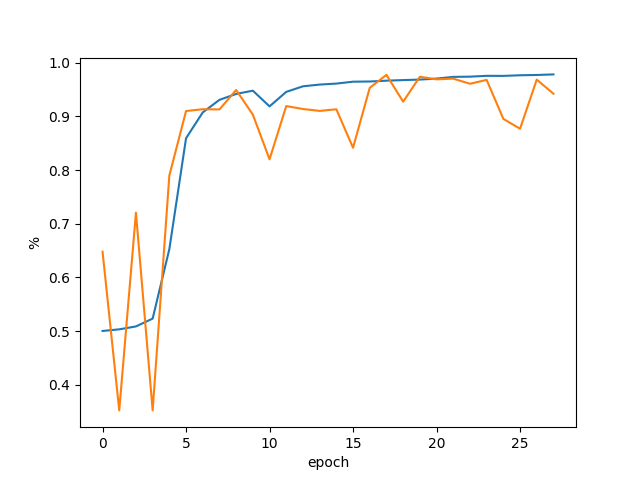
\includegraphics[scale=.6]{image/chapter6/acc.png}
    \begin{figure}[htp]
    \begin{center}
    \end{center}
    \caption{Độ chính xác của quá trình huấn luyện và kiểm thử}
    \end{figure}
\end{center}
\begin{center}
    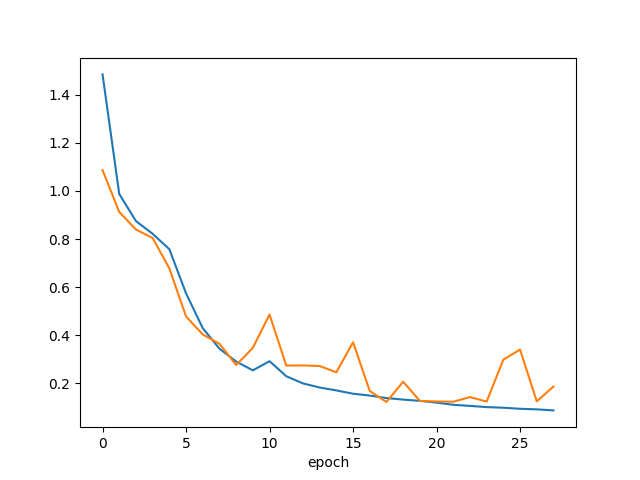
\includegraphics[scale=.6]{image/chapter6/loss.png}
    \begin{figure}[htp]
    \begin{center}
    \end{center}
    \caption{Độ mất mát của quá trình huấn luyện và kiểm thử}
    \end{figure}
\end{center}

\subsection{Phân loại trên 20 đoạn RR liên tiếp}
\subsubsection{Chia tập dữ liệu}
\begin{center}
    \begin{tabular}{|c|c|}
    \hline 
    Tập dữ liệu huấn luyện & Tập dữ liệu kiểm thử \\ 
    \hline 
    37623 & 44034\\
    \hline 
    \end{tabular}
\end{center}
\subsubsection{Kết quả}
Kết quả được đánh giá theo độ đo: Precision, Recall, F1-score, Accuracy, Loss.
\begin{center}
    \begin{tabular}{|c|c|c|}
    \hline
    Estimate & Normal & Abnormal\\
    \hline 
    Precision & 0.96 & 0.74\\ 
    \hline 
    Recall & 0.87 & 0.92\\
    \hline 
    F1-score & 0.90 & 0.81\\
    \hline 
    Accuracy & \multicolumn{2}{|c|}{0.95} \\
    \hline 
    Loss & \multicolumn{2}{|c|}{0.03} \\
    \hline
    \end{tabular}
\end{center}
\begin{center}
    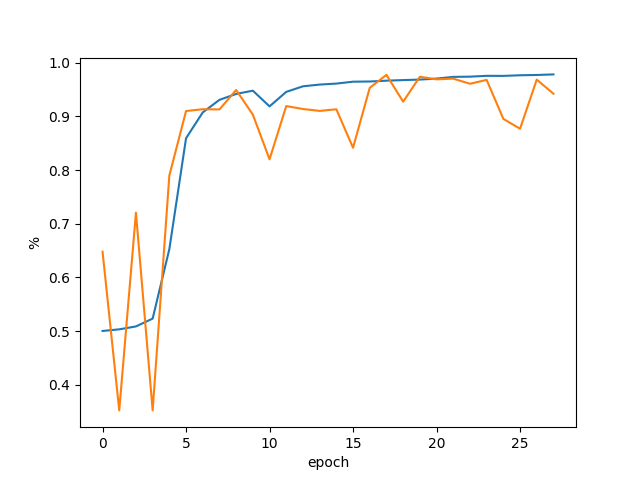
\includegraphics[scale=.6]{image/chapter6/acc.png}
    \begin{figure}[htp]
    \begin{center}
    \end{center}
    \caption{Độ chính xác của quá trình huấn luyện và kiểm thử}
    \end{figure}
\end{center}
\begin{center}
    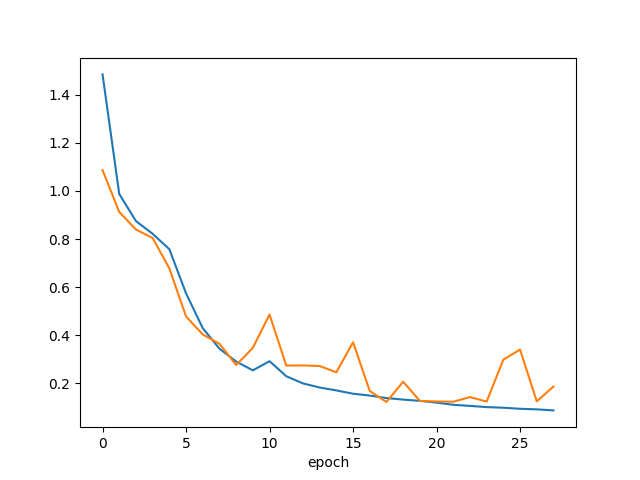
\includegraphics[scale=.6]{image/chapter6/loss.png}
    \begin{figure}[htp]
    \begin{center}
    \end{center}
    \caption{Độ mất mát của quá trình huấn luyện và kiểm thử}
    \end{figure}
\end{center}

\section{Thảo luận}
Nghiên cứu đã thực hiện phân loại tín hiệu điện tâm đồ bằng mạng Trí nhớ ngắn dài 
